\begin{frame}{}
    \LARGE SSL: \textbf{Instance Discrimination \& Contrastive Learning}
\end{frame}

\begin{frame}[t,allowframebreaks]{Instance Discrimination \& Contrastive Learning }
    \textbf{Pretext Task Evolution:}
    \begin{itemize}
        \item Earlier: handcrafted tasks (e.g., jigsaw, colorization).
        \item Now: contrastive learning directly optimizes for invariance and discrimination.
        \item Leads to better, more transferable features and narrows the gap with supervised learning.
    \end{itemize}

    \framebreak

    \textbf{Instance Discrimination:}
    \begin{itemize}
        \item Treats each image as its own class.
        \item Positive pairs: augmented views of the same image.
        \item Negative pairs: views from different images.
        \item Promotes invariance to augmentations and discrimination between instances.
    \end{itemize}

    \vspace{0.5em}

    \textbf{Contrastive Learning:}
    \begin{itemize}
        \item Self-supervised approach for learning representations, especially in vision.
        \item Uses data structure instead of labels.
        \item Learns by pulling together similar (positive) pairs and pushing apart dissimilar (negative) pairs using a contrastive loss (e.g., InfoNCE).
    \end{itemize}
\end{frame}

\subsection{Instance Discrimination}
\begin{frame}[allowframebreaks]{Fundamentals of Instance Discrimination}
    \textbf{Instance Discrimination} is a self-supervised learning approach where each individual sample in the dataset is treated as a distinct class.
    \begin{itemize}
        \item The core idea is to learn representations by distinguishing between different instances, rather than relying on human-annotated labels.
        \item \textbf{Positive pairs} are generated by applying different augmentations (such as cropping, color jittering, or flipping) to the same image. These augmented views are considered to belong to the same class (i.e., the same instance).
        \item \textbf{Negative pairs} are formed by pairing augmented views of different images. These are treated as belonging to different classes (i.e., different instances).
    \end{itemize}

    \framebreak
    \begin{figure}
        \centering
        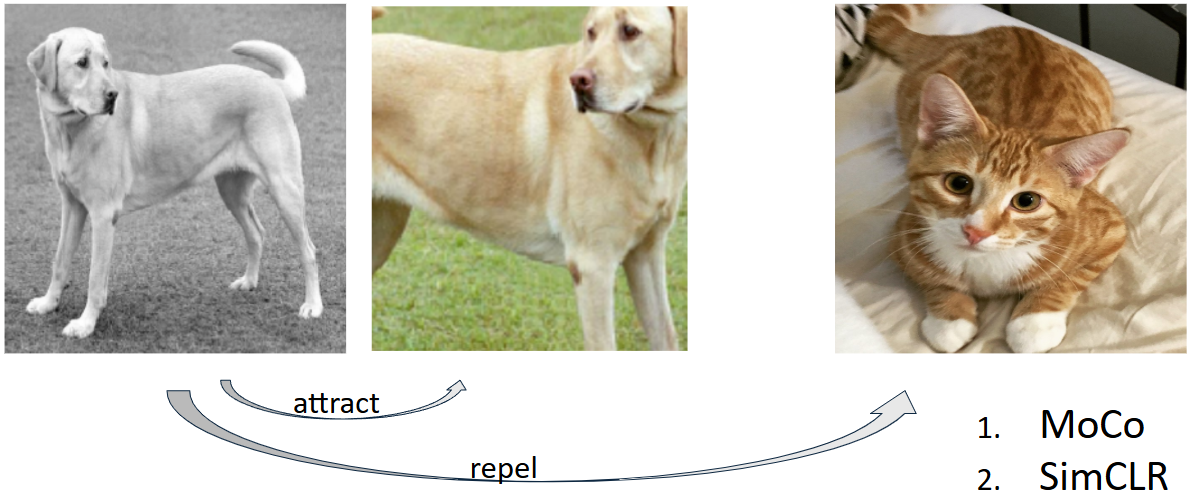
\includegraphics[width=1\linewidth,height=0.9\textheight,keepaspectratio]{images/ssl/slide_63_img.png}
        % \footnote{Wu et al (2018). Unsupervised Feature Learning via Non-Parametric Instance Discrimination. CVPR 2018.}
    \end{figure}

    \framebreak
    \begin{itemize}
        \item The learning objective is to \textbf{maximize agreement} (similarity) between representations of positive pairs, while minimizing agreement between negative pairs.
        \item This is typically achieved using a contrastive loss function, such as InfoNCE, which encourages the model to bring positive pairs closer in the embedding space and push negative pairs apart.
        \item Instance discrimination forms the basis for many popular self-supervised learning methods, such as MoCo, SimCLR, and PIRL.
        \item By maximizing agreement across views of the same instance, the model learns to extract meaningful and invariant features, which can be transferred to downstream tasks.
    \end{itemize}
\end{frame}
\subsection{Momentum Contrast (MoCo)}
\begin{frame}[allowframebreaks]{Momentum Contrast (MoCo)}
    \begin{figure}
        \centering
        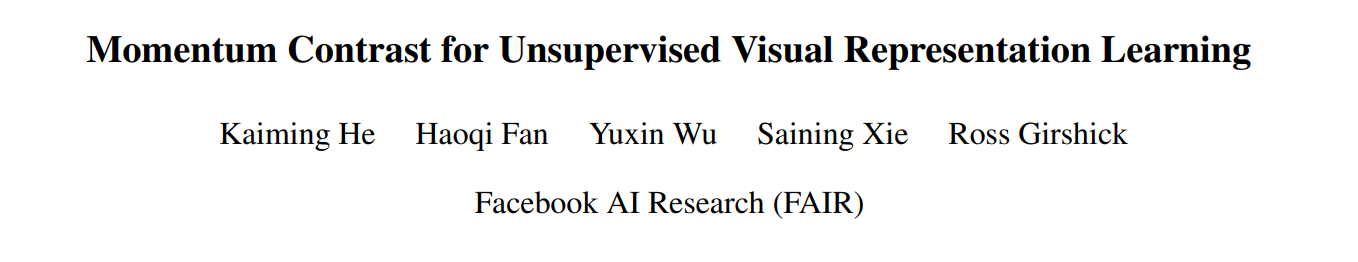
\includegraphics[width=1\linewidth,height=0.9\textheight,keepaspectratio]{images/ssl/slide_65_1_img.png}
    \end{figure}

    \framebreak

    \textbf{Momentum Contrast (MoCo)} is a self-supervised learning framework designed for visual representation learning. Its key components are:

    \vspace{0.5em}

    \textbf{Query \& Key Encoders}: Two neural networks, $f_q$ (query encoder) and $f_k$ (key encoder), are used. The key encoder $f_k$ is updated as an exponential moving average of the query encoder $f_q$:
        \[
            \theta_k \leftarrow m \theta_k + (1 - m) \theta_q
        \]
        where $\theta_k$ and $\theta_q$ are the parameters of $f_k$ and $f_q$, and $m$ is the momentum coefficient (e.g., $m=0.999$).
    
    \framebreak

    \begin{figure}
        \centering
        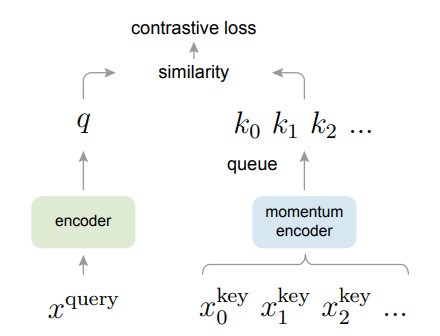
\includegraphics[width=1\linewidth,height=0.9\textheight,keepaspectratio]{images/ssl/slide_66_1_img.png}
    \end{figure}

    \framebreak

    \textbf{Dictionary Queue}: MoCo maintains a large queue (dictionary) of encoded keys from previous batches. This enables the use of a large and consistent set of negative samples for contrastive learning, which is crucial for effective representation learning.
    
    \vspace{0.5em}
    
    \textbf{Contrastive Loss}: The InfoNCE loss is used to train the encoders. For a given query $q$ and its positive key $k^+$, along with a set of negative keys $\{k_0, k_1, ..., k_N\}$ from the dictionary, the loss is:
        \[
            \mathcal{L}_{q} = -\log \frac{\exp(q \cdot k^+ / \tau)}{\exp(q \cdot k^+ / \tau) + \sum_{i=0}^{N} \exp(q \cdot k_i / \tau)}
        \]
        where $\tau$ is a temperature hyperparameter.

    \framebreak

    \begin{columns}
        \column{0.5\textwidth}
            \begin{figure}
                \centering
                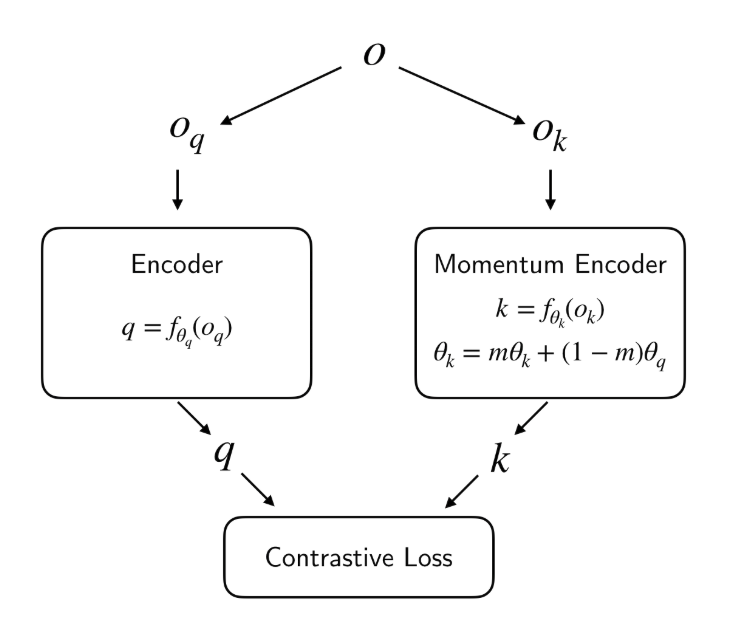
\includegraphics[width=1\linewidth,height=0.9\textheight,keepaspectratio]{images/ssl/slide_67_1_img.png}
            \end{figure}
        \column{0.5\textwidth}
            \begin{figure}
                \centering
                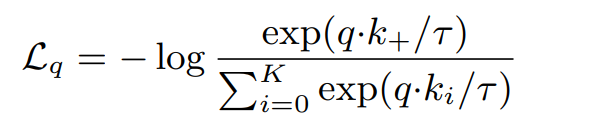
\includegraphics[width=1\linewidth,height=0.9\textheight,keepaspectratio]{images/ssl/slide_67_2_img.png}
            \end{figure}
    \end{columns}
    \framebreak

    \textbf{Key Steps in MoCo Training:}
    \begin{enumerate}
        \item For each image, generate two augmentations: one for the query encoder ($f_q$), one for the key encoder ($f_k$).
        \item Encode the query and key.
        \item Compute the InfoNCE loss using the current positive key and the dictionary of negative keys.
        \item Update $f_q$ via backpropagation; update $f_k$ via momentum.
        \item Enqueue the new key and dequeue the oldest key to maintain the dictionary size.
    \end{enumerate}

    \framebreak

    \begin{figure}
        \centering
        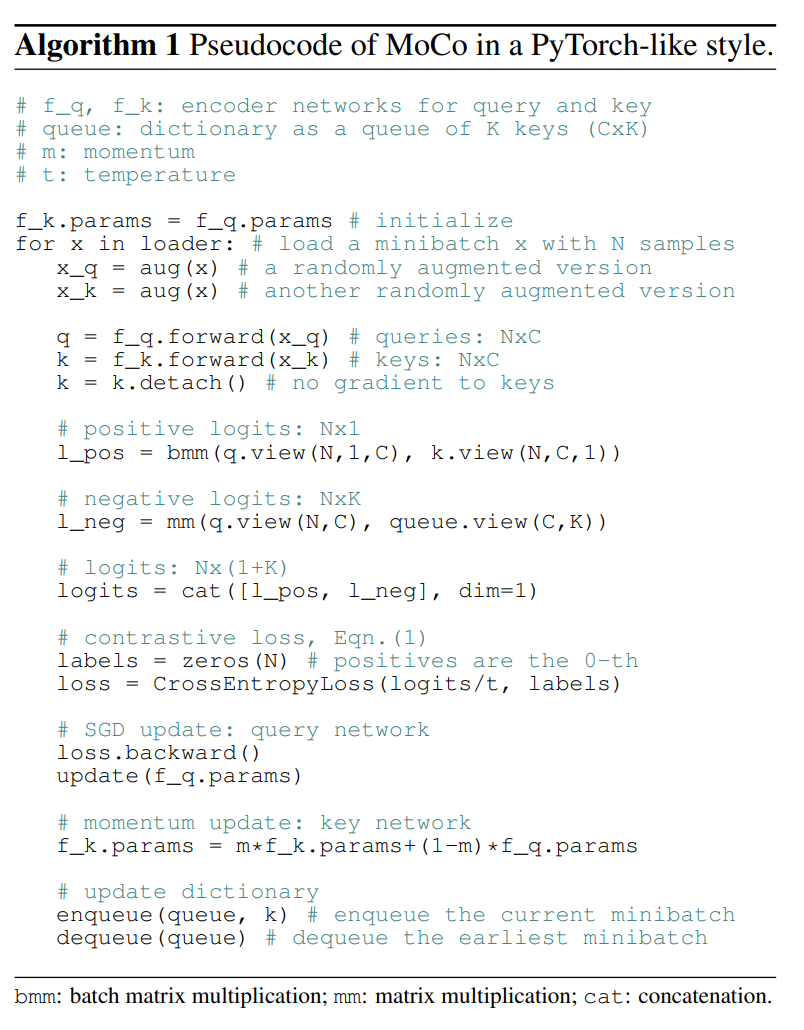
\includegraphics[width=1\linewidth,height=0.95\textheight,keepaspectratio]{images/ssl/slide_68_1_img.png}
    \end{figure}

    \framebreak

    \begin{figure}
        \centering
        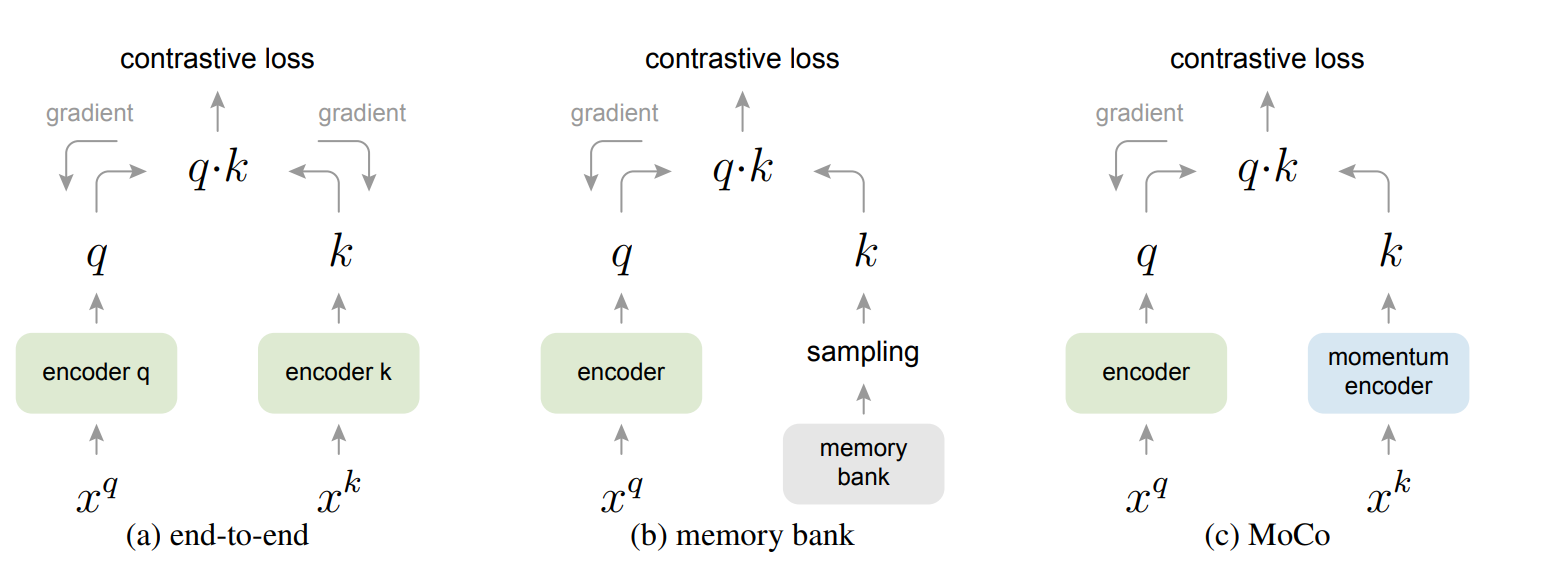
\includegraphics[width=1\linewidth,height=0.95\textheight,keepaspectratio]{images/ssl/slide_69_1_img.png}
    \end{figure}

    \framebreak

    \begin{figure}
        \centering
        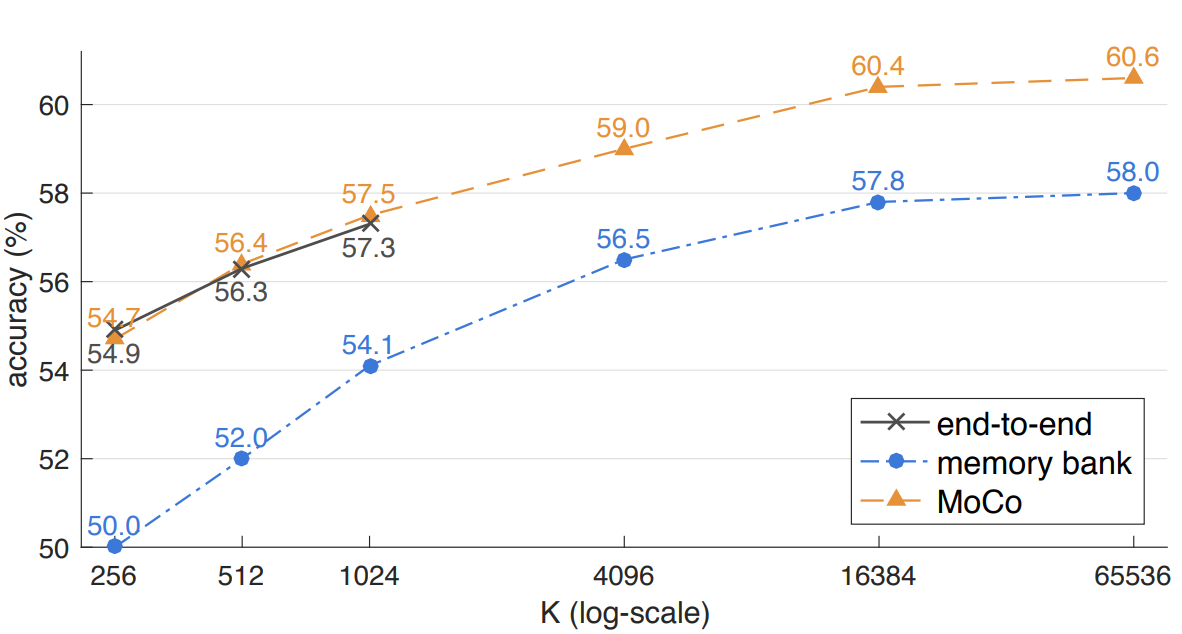
\includegraphics[width=1\linewidth,height=0.95\textheight,keepaspectratio]{images/ssl/slide_70_1_img.png}
    \end{figure}

    \framebreak

    \begin{figure}
        \centering
        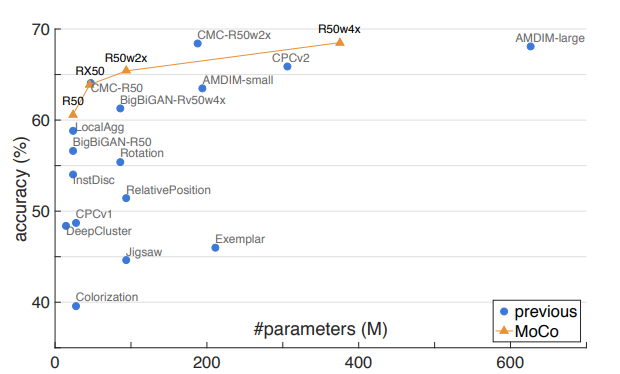
\includegraphics[width=1\linewidth,height=0.95\textheight,keepaspectratio]{images/ssl/slide_71_1_img.png}
    \end{figure}

    \framebreak

    \textbf{Key Advantages:}
    \begin{itemize}
        \item Enables large and consistent negative sets for contrastive learning.
        \item Momentum update stabilizes the key encoder, improving training.
        \item Scalable to large datasets and high-dimensional representations.
    \end{itemize}
\end{frame}